\newcommand{\svcourse}{CST Part IA: Software Engineering and Security}
\newcommand{\svnumber}{1}
\newcommand{\svvenue}{Microsoft Teams}
\newcommand{\svdate}{2022-05-11}
\newcommand{\svtime}{15:00}
\newcommand{\svuploadkey}{CBd13xmL7PC1zqhNIoLdTiYUBnxZhzRAtJxv/ytRdM1r7qIfwMsxeVwM/pPcIo8l}

\newcommand{\svrname}{Dr Sam Ainsworth}
\newcommand{\jkfside}{oneside}
\newcommand{\jkfhanded}{yes}

\newcommand{\studentname}{Harry Langford}
\newcommand{\studentemail}{hjel2@cam.ac.uk}


\documentclass[10pt,\jkfside,a4paper]{article}

% DO NOT add \usepackage commands here.  Place any custom commands
% into your SV work files.  Anything in the template directory is
% likely to be overwritten!

\usepackage{fancyhdr}

\usepackage{lastpage}       % ``n of m'' page numbering
\usepackage{lscape}         % Makes landscape easier

\usepackage{verbatim}       % Verbatim blocks
\usepackage{listings}       % Source code listings
\usepackage{epsfig}         % Embed encapsulated postscript
\usepackage{array}          % Array environment
\usepackage{qrcode}         % QR codes
\usepackage{enumitem}       % Required by Tom Johnson's exam question header

\usepackage{hhline}         % Horizontal lines in tables
\usepackage{siunitx}        % Correct spacing of units
\usepackage{amsmath}        % American Mathematical Society
\usepackage{amssymb}        % Maths symbols
\usepackage{amsthm}         % Theorems

\usepackage{ifthen}         % Conditional processing in tex

\usepackage[top=3cm,
            bottom=3cm,
            inner=2cm,
            outer=5cm]{geometry}

% PDF metadata + URL formatting
\usepackage[
            pdfauthor={\studentname},
            pdftitle={\svcourse, SV \svnumber},
            pdfsubject={},
            pdfkeywords={9d2547b00aba40b58fa0378774f72ee6},
            pdfproducer={},
            pdfcreator={},
            hidelinks]{hyperref}


% DO NOT add \usepackage commands here.  Place any custom commands
% into your SV work files.  Anything in the template directory is
% likely to be overwritten!

\usepackage{fancyhdr}

\usepackage{lastpage}       % ``n of m'' page numbering
\usepackage{lscape}         % Makes landscape easier

\usepackage{verbatim}       % Verbatim blocks
\usepackage{listings}       % Source code listings
\usepackage{graphicx}
\usepackage{float}
\usepackage{epsfig}         % Embed encapsulated postscript
\usepackage{array}          % Array environment
\usepackage{qrcode}         % QR codes
\usepackage{enumitem}       % Required by Tom Johnson's exam question header

\usepackage{hhline}         % Horizontal lines in tables
\usepackage{siunitx}        % Correct spacing of units
\usepackage{amsmath}        % American Mathematical Society
\usepackage{amssymb}        % Maths symbols
\usepackage{amsthm}         % Theorems

\usepackage{ifthen}         % Conditional processing in tex

\usepackage[top=3cm,
            bottom=3cm,
            inner=2cm,
            outer=5cm]{geometry}

% PDF metadata + URL formatting
\usepackage[
            pdfauthor={\studentname},
            pdftitle={\svcourse, SV \svnumber},
            pdfsubject={},
            pdfkeywords={9d2547b00aba40b58fa0378774f72ee6},
            pdfproducer={},
            pdfcreator={},
            hidelinks]{hyperref}

\renewcommand{\headrulewidth}{0.4pt}
\renewcommand{\footrulewidth}{0.4pt}
\fancyheadoffset[LO,LE,RO,RE]{0pt}
\fancyfootoffset[LO,LE,RO,RE]{0pt}
\pagestyle{fancy}
\fancyhead{}
\fancyhead[LO,RE]{{\bfseries \studentname}\\\studentemail}
\fancyhead[RO,LE]{{\bfseries \svcourse, SV~\svnumber}\\\svdate\ \svtime, \svvenue}
\fancyfoot{}
\fancyfoot[LO,RE]{For: \svrname}
\fancyfoot[RO,LE]{\today\hspace{1cm}\thepage\ / \pageref{LastPage}}
\fancyfoot[C]{\qrcode[height=0.8cm]{\svuploadkey}}
\setlength{\headheight}{22.55pt}


\ifthenelse{\equal{\jkfside}{oneside}}{

 \ifthenelse{\equal{\jkfhanded}{left}}{
  % 1. Left-handed marker, one-sided printing or e-marking, use oneside and...
  \evensidemargin=\oddsidemargin
  \oddsidemargin=73pt
  \setlength{\marginparwidth}{111pt}
  \setlength{\marginparsep}{-\marginparsep}
  \addtolength{\marginparsep}{-\textwidth}
  \addtolength{\marginparsep}{-\marginparwidth}
 }{
  % 2. Right-handed marker, one-sided printing or e-marking, use oneside.
  \setlength{\marginparwidth}{111pt}
 }

}{
 % 3. Alternating margins, two-sided printing, use twoside.
}


\setlength{\parindent}{0em}
\addtolength{\parskip}{1ex}

% Exam question headings, labels and sensible layout (courtesy of Tom Johnson)
\setlist{parsep=\parskip, listparindent=\parindent}
\newcommand{\examhead}[3]{\section{#1 Paper #2 Question #3}}
\newenvironment{examquestion}[3]{
\examhead{#1}{#2}{#3}\setlist[enumerate, 1]{label=(\alph*)}\setlist[enumerate, 2]{label=(\roman*)}
\marginpar{\href{https://www.cl.cam.ac.uk/teaching/exams/pastpapers/y#1p#2q#3.pdf}{\qrcode{https://www.cl.cam.ac.uk/teaching/exams/pastpapers/y#1p#2q#3.pdf}}}
\marginpar{\footnotesize \href{https://www.cl.cam.ac.uk/teaching/exams/pastpapers/y#1p#2q#3.pdf}{https://www.cl.cam.ac.uk/\\teaching/exams/pastpapers/\\y#1p#2q#3.pdf}}
}{}


\usepackage{listings}
\usepackage{tikz}
\usepackage{enumitem}
\usepackage{graphicx}
\graphicspath{ {./images/}}

\lstdefinestyle{py}{
  belowcaptionskip=1\baselineskip,
  breaklines=true,
  xleftmargin=\parindent,
  language=python,
  showstringspaces=false,
  basicstyle=\footnotesize\ttfamily,
  keywordstyle=\bfseries\color{orange!80!black},
  commentstyle=\itshape\color{green40!black},
  stringstyle=\color{green!40!black},
}

\lstdefinestyle{jav}{
  belowcaptionskip=1\baselineskip,
  breaklines=true,
  xleftmargin=\parindent,
  language=java,
  showstringspaces=false,
  basicstyle=\footnotesize\ttfamily,
  keywordstyle=\bfseries\color{orange!80!black},
  commentstyle=\itshape\color{green!40!black},
  stringstyle=\color{green!40!black},
}


\begin{document}

\section{Fibonacci Heaps}

\begin{enumerate}

\item Describe the structure of a node in a Fibonacci heap and why each field is required.
Hints:

A fib-heap node has 8 fields.

\begin{itemize}

\item the key of the node

The metric which we are finding the minimum of -- the ``priority'' of the value stored in 
the node.

\item the value of the node (or a pointer to the value)

The value we wish to retrieve.

\item boolean to mark the node as loser or not

To ensure fibonacci trees are sufficiently deep we must remove nodes from their trees and 
place them into the root list when two of their children are removed. After their first 
child is removed we mark them as losers.

\item pointer to the nodes parent

When we call {\tt decrease\_key} (and indirectly, delete) we must access the parent in constant 
time to check whether the childs key is now less than the parents key. A pointer to the 
parent allows us to do this.

\item pointer to one child

In {\tt pop\_min}, we promote all the minimum nodes children to the root. To do this we must 
iterate through the list of children. So we must be able to reach the children. Note that 
since all the children are linked to each other, we only need a pointer to \textit{one} child. 

When merging trees in {\tt cleanup} we insert the root with the 
larger key into the child list of the other root. Note again that this only needs a pointer 
to \textit{one} child.

\item integer holding the degree of the node (the number of children that node has)

In {\tt cleanup} trees are merged with trees of the same degree. So we need to know 
the degree of nodes in constant time -- otherwise {\tt cleanup} would be $O((\lg n)^2)$ 
rather than $O(\lg n)$. So we store each nodes' degree.

\item pointer to left sibling

This connects the roots (or children) into a linked list. 
Dependent on whether the node is in the root list or not, this either allows us to iterate 
through child lists or the root list.

\item pointer to right sibling

This turns the linked list into a circular linked list allowing splicing from the linked list 
in constant time given a node. This is needed in {\tt decrease\_key} to remove the node we 
are passed and loser nodes.

\end{itemize}

\item Explain how to create an empty Fibonacci heap, and state the big-O cost.

Create a new fibonacci heap object which has a null {\tt min\_node}, an empty 
root list and zero size. This has $\Theta(1)$ time complexity.

\item Explain how to add one new key/value pair into an existing Fibonacci heap, and state the big-O
cost.

Create a new node which holds the key-value pair with all other fields 
set to 0 or null as appropriate. Then insert it into the root list by changing four pointers -- 
the new nodes left and right pointers and two adjacent nodes left and right pointers. 
This has $\Theta(1)$ time and space complexity.

\item Explain how to form the (destructive) union of two existing Fibonacci heaps, and state the
big-O cost.

Create a new fibonacci heap with {\tt min\_node} as the of the smaller of the two existing 
Fibonacci Heaps {\tt min\_node}. Then splice the linked lists of the two Fibonacci Heaps together. 
If you store the size of the Fibonacci Heap, (which makes the code faster and simpler but is not 
necessary) then set the new Fibonacci Heaps size equal to the two old Fibonacci Heap's size. 
Both these operations require constant time and space.

\item Explain how to identify the smallest item in a Fibonacci heap, and state the big-O cost.

We keep a pointer to the {\tt min\_node} in the Fibonacci Heap. So identification of the 
smallest item in a Fibonacci Heap involves returning a pointer to the {\tt min\_node} -- or 
the value of the {\tt min\_node} dependent on implementation.

\textit{Removal} of the {\tt min\_node} in the Fibonacci Heap is more complicated.

\begin{itemize}

\item Find the {\tt min\_node}. 

This has $\Theta(1)$ space and time complexity.

\item Promote all of {\tt min\_node}'s children into the root list. 

To do this we splice the child list into the root list and change each parent pointer 
to point to null -- or to keep the Fibonacci Heap in a consistent state throughout, insert 
each node one-by-one into the root list.

Both have constant space complexity and 
time complexity $\Theta(d)$ where $d$ is the degree of {\tt min\_node} and $d \in O(\lg n)$.

So the space complexity is $\Theta(1)$ and the time complexity is $O(\lg n)$.

\item Clean up the root list. 

To do this we create an array of pointers of size $d_{\text{max}}$ where $d_{\text{max}}$ is the largest 
possible degree of a node in the Fibonacci Heap. $d_{\text{max}} \in \Theta(\lg n)$. So the space 
complexity of this algorithm is $\Theta(\lg n)$.

For each root in the root list, let $d$ be the degree of the root. Check the $d^\text{th}$ position 
in the array. 

If it is null then there is no root of size $d$ in the array. In this case we should 
set the $d^\text{th}$ position in the array to point to this root. 

Else we should merge this tree with the tree at position $d$ and check the merged tree against position $d + 1$.
We merge the two trees by comparing the roots and inserting tree with the larger root into the child 
list of the tree with the smaller root.

This has space complexity $\Theta(\lg n)$ and ammortized time complexity of $\Theta(\lg n)$ -- although a 
worst-case individual time complexity of $O(n)$.

\item Then parse through the new root list to find the {\tt min\_node}.

This has space complexity $\Theta(1)$ and time complexity $\Theta(\lg n)$.

\end{itemize}

So {\tt pop\_min} has space complexity $\Theta(\lg n)$ and ammortized time complexity $\Theta(\lg n)$.

\end{enumerate}

I implemented a Fibonacci Heap in Java as part of the learning process for this supervision. 
However the code is (5.5 pages) long so I won't include it.

\newpage

\section{Convex Hulls}

\begin{enumerate}

\item Describe how to determine whether or not a point is inside a simple plane 
closed polygon, paying proper attention to awkward cases.

\subsection{Ray Tracing}

If a point $P$ is inside a closed polygon then any vector from that point to 
outside the polygon will intersect an odd number of lines.

Firstly, find a point $Q$ which is outside the polygon. An easy way to do this is 
by considering the point $Q = \begin{pmatrix} x_{\text{max}}.x + \delta \\ 
x_{\text{max}}.y \\ \end{pmatrix}$ where $\delta$ is an arbitrary positive 
constant.

For each line on the surface of the polygon, check whether the line $PQ$ intersects it. 

If the number of edges the $PQ$ intersects is even then $P$ is inside the polygon 
otherwise $P$ is outside the polygon.

\vspace{0.1cm}

We can check whether $\overrightarrow{AB}$ intersects $\overrightarrow{PQ}$ with the following routine:

Check whether $A$ and $B$ are on opposite sides of the line $\overrightarrow{PQ}$ and 
whether $P$ and $Q$ are on opposite sides of the line $\overrightarrow{AB}$. If both are 
true then the lines intersect.

Given the line $\overrightarrow{AB}$ and points $P$, $Q$ we can check whether $A$ and $B$ are on 
opposite sides of $\overrightarrow{PQ}$ by working out a line $\overrightarrow{\ell} \perp \overrightarrow{PQ}$. 
If $A\cdot \overrightarrow{\ell} - P\cdot \overrightarrow{\ell}$ has an opposite sign to $B\cdot \overrightarrow{\ell} - P \cdot \overrightarrow{\ell}$ 
then the points are on the opposite sides of the line. 

We repeat this for the points $P$, $Q$ and the line $\overrightarrow{AB}$.

\item Describe how, with luck, to exclude large numbers of points from the convex hull 
of a set of points in the plane, with due consideration of what can go wrong.

The easiest way to ``with luck'' remove a large set of points is to get 
$x_{\min}, x_{\max}, y_{\min}, y_{\max}$ and remove any points in the square 
formed by those four vertices.

This works because all four of these vertices are on the convex hull and no point 
which is bounded by points on the convex hull can possibly be on the convex hull. 
So all points which are bounded by the square formed by these four points are known 
not to be on the convex hull. This optimisation is linear and will remove at least half 
the area of the graph from consideration on the convex hull. On ``fairly'' uniform 
graphs this will remove around half of the points in the graph.

However this has no affect on the expected complexity. The following algorithm does:

\vspace{0.3cm}

\subsection*{Abstract}

I extended this idea by reinventing ($\dag$) a vectorisable expected $O(n)$ 
(but $O(nh)$ worst-case) convex-hull algorithm and adding 
termination conditions if it starts performing worse than $O(n)$. After 
implementing this algorithm I found that it was able to speed up 
scipy.spatial.ConvexHull on graphs with a ``low'' proportion of points near the 
convex hull and made little difference on non-adversarial graphs.

On non-adversarial graphs the termination conditions are very unlikely to trigger; 
this means that on non-adversarial graphs the complexity of finding the 
convex hull is now $O(n + h \lg h)$ expected (although the worst-case is unchanged).

($\dag$) At the time of writing I believed that the algorithm the filtering 
is based on was original but have since found out it already existed and is called 
``Quickhull''. The adaptation to use it to filter points and everything written 
here is my own.

\vspace{0.3cm}

\subsection*{Outline}

The summary of the filtering algorithm is as follows:

\begin{itemize}

\item Split the graph with a line from $x_\text{min}$ to $x_\text{max}$.

\item Find the point with the largest perpendicular distance onto the line and 
remove all points bounded by it and the two end points. Recurse down each edge and 
repeat until there are no points in the edge or insufficient points are removed.

\end{itemize}

Here is a more in-depth outline.

\begin{enumerate}[label=(\alph*)]

\item Find the point with the largest $x$ coordinate ($x_\text{max}$) and the point with the smallest $x$ coordinate 
($x_\text{min}$). If these points have the same $x$ coordinate then the graph is degenerate and there is no 
convex hull.

\item Draw a line $L$ joining $x_\text{max}$ and $x_\text{min}$.

\item Split the graph into those points above $L$ and those points below $L$.

\item For those points above the line $L$:

\item Find the point $P$ which has the largest projection onto the line perpendicular to $L$. 
$P$ is on the convex hull. Remove all points bounded by $P$ and $L$ using the method described 
above.

\item Split the points into those to the right of the convex-hull point $D$ we have just found 
and those to the left of the convex-hull point $G$. We can combine this calculation with elimination 
of points bounded by $P$ and $L$.

\item If this call has not removed at least 25\% of points then mark the next recursive call with kill=True. 
If this recursive call already had kill=True then do not recurse further. This ensures linear complexity.

\item Repeat steps (e) - (i) for the points in $D$ considering the line formed by $P$ and 
the right point of $L$ as $L$.

\item Repeat steps (e) - (i) for the points in $G$ considering the line formed by $P$ and 
the left point of $L$ as $L$.

\item Repeat steps (d) - (i) for those points below the line $L$ between $x_\text{min}$ and $x_\text{max}$.

\end{enumerate}

Here are several graphs illustrating three things: 

\begin{itemize}

\item On graphs with a low proportion of points on the convex hull, this algorithm 
speeds up even highly optimised implementations.

\item On non-adversarial graphs the filtering removes the overwhelming majority of points 
which are not on the convex hull. This is shown by how much quicker ConvexHull is after 
the filtering.

\item The complexity is linear.

\end{itemize}

In the following graph ``filtering'' is the time the point filtering took, 
``Filtered ConvexHull'' is the time taken to filter the points and then call 
scipy.spatial.ConvexHull and ``ConvexHull'' is the time taken to run scipy.spatial.ConvexHull 
without any filtering.

Typical graph with a low proportion of points on the convex hull 
(random angle with radius $r$ normally distributed $r \sim N(1, 0.5^2$)):
\begin{center}
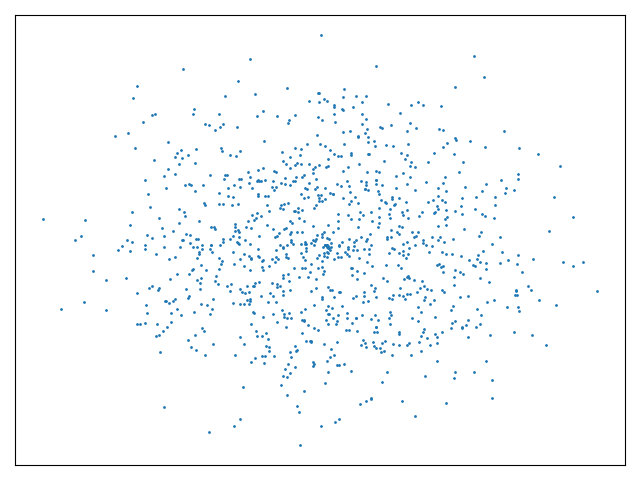
\includegraphics[width=5cm]{normalvariate}
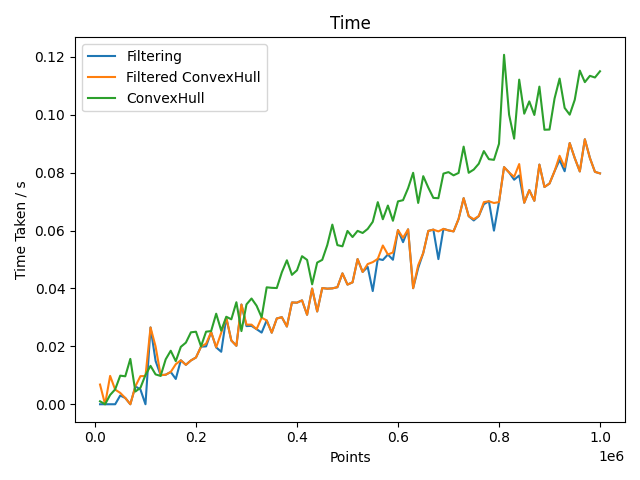
\includegraphics[width=5cm]{normalvariate_times}
\end{center}

Random uniformly distributed within a circle (high proportion of points on the convex hull):
\begin{center}
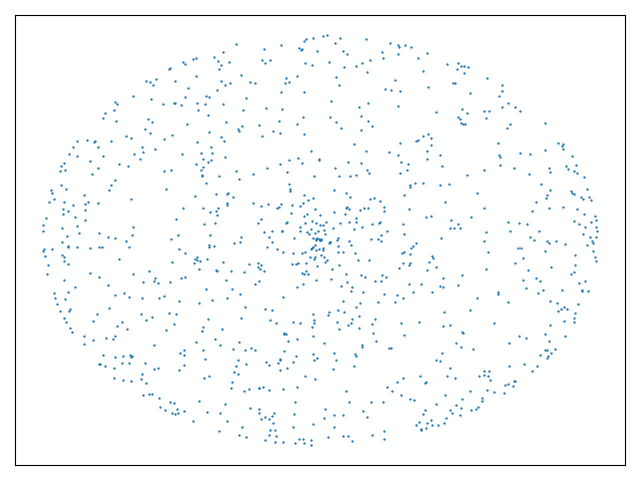
\includegraphics[width=5cm]{circle_points}
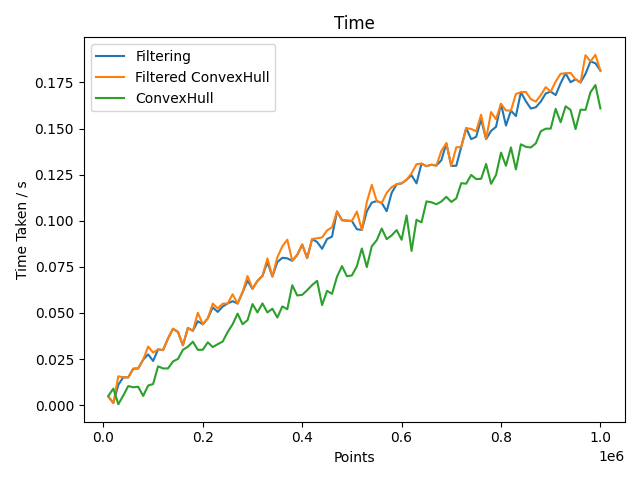
\includegraphics[width=5cm]{circleraw}
\end{center}

Here is a degenerate case all the points are on the surface of the circle and so 
all points are on the convex hull:
\begin{center}
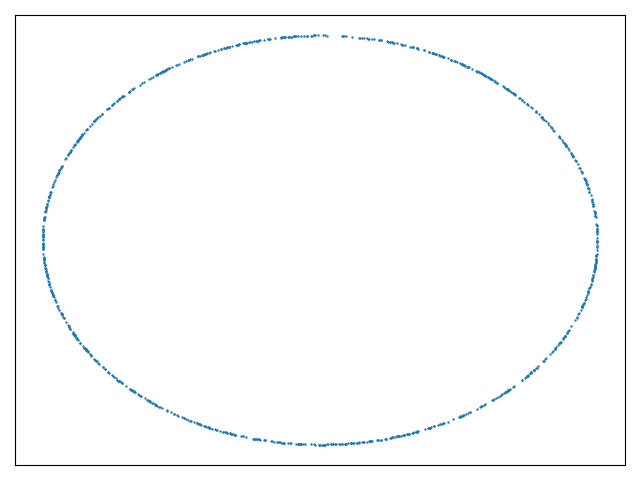
\includegraphics[width=5cm]{circlesurface}
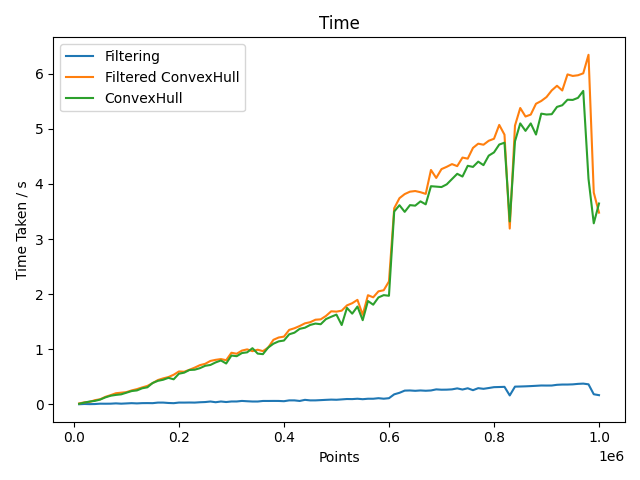
\includegraphics[width=5cm]{surface_points}
\end{center}

\subsection*{Worked Example}

After finding a node is on the convex hull, I will colour it blue. If I find that a node 
cannot possibly be on the convex hull, I will colour it light gray.
I will also perform all the executions at the $i^\text{th}$ level at once for demonstration 
purposes -- in reality these are not done in parallel.

Start with the graph as below.

\begin{center}
\begin{tikzpicture}[xscale=0.5, yscale=0.5]
\node (x0) at (4.093442680978736, 0.41889336196670435) {$x_{0}$};
\node (x1) at (6.615665555666604, 6.1896116481505175) {$x_{1}$};
\node (x2) at (3.8779690768063997, 5.211040980314668) {$x_{2}$};
\node [blue] (x3) at (7.799915473235454, 4.4212567328378904) {$x_{3}$};
\node (x4) at (3.6097913305830653, 7.773417517032471) {$x_{4}$};
\node (x5) at (7.041368600618052, 6.6226789311846845) {$x_{5}$};
\node (x6) at (0.23111663120234027, 7.636702820626231) {$x_{6}$};
\node [blue] (x7) at (0.03003578218411551, 5.8543935696002425) {$x_{7}$};
\node (x8) at (3.0093922230982875, 4.078598305143715) {$x_{8}$};
\node (x9) at (7.600374365675198, 2.9923212115279334) {$x_{9}$};
\node (x10) at (1.5232292361242585, 3.405026159301018) {$x_{10}$};
\node (x11) at (5.064692465334404, 4.651468145006333) {$x_{11}$};
\node (x12) at (3.3609099677756378, 5.3363875228012665) {$x_{12}$};
\node (x13) at (3.2369922175066526, 2.2429433965775543) {$x_{13}$};
\node (x14) at (2.8888152617406098, 2.4874016292731875) {$x_{14}$};
\node (x15) at (6.711765453935924, 7.296148293105408) {$x_{15}$};
\node (x16) at (4.950081975558071, 7.568427769499155) {$x_{16}$};
\node (x17) at (4.336177552023418, 6.164732525032696) {$x_{17}$};
\node (x18) at (4.865988864577287, 0.6142255644992014) {$x_{18}$};
\node (x19) at (3.1982495211858186, 6.621414130050312) {$x_{19}$};
\end{tikzpicture}
\end{center}

Firstly we join the rightmost and leftmost nodes together. These nodes 
are guaranteed to be on the convex hull. We should project all the points 
onto the vector perpendicular to this line and form a triangle from the 
point which is the greatest distance from this line in each partition.

We then note that all the points enclosed by either triangle must 
not be on the convex hull. So we can remove them.

\begin{center}
\begin{tikzpicture}[xscale=0.5, yscale=0.5]
\node [blue] (x0) at (4.093442680978736, 0.41889336196670435) {$x_{0}$};
\node [lightgray] (x1) at (6.615665555666604, 6.1896116481505175) {$x_{1}$};
\node [lightgray] (x2) at (3.8779690768063997, 5.211040980314668) {$x_{2}$};
\node [blue] (x3) at (7.799915473235454, 4.4212567328378904) {$x_{3}$};
\node (x4) at (3.6097913305830653, 7.773417517032471) {$x_{4}$};
\node [lightgray] (x5) at (7.041368600618052, 6.6226789311846845) {$x_{5}$};
\node (x6) at (0.23111663120234027, 7.636702820626231) {$x_{6}$};
\node [blue] (x7) at (0.03003578218411551, 5.8543935696002425) {$x_{7}$};
\node [lightgray] (x8) at (3.0093922230982875, 4.078598305143715) {$x_{8}$};
\node (x9) at (7.600374365675198, 2.9923212115279334) {$x_{9}$};
\node (x10) at (1.5232292361242585, 3.405026159301018) {$x_{10}$};
\node [lightgray] (x11) at (5.064692465334404, 4.651468145006333) {$x_{11}$};
\node [lightgray] (x12) at (3.3609099677756378, 5.3363875228012665) {$x_{12}$};
\node [lightgray] (x13) at (3.2369922175066526, 2.2429433965775543) {$x_{13}$};
\node [lightgray] (x14) at (2.8888152617406098, 2.4874016292731875) {$x_{14}$};
\node [blue] (x15) at (6.711765453935924, 7.296148293105408) {$x_{15}$};
\node (x16) at (4.950081975558071, 7.568427769499155) {$x_{16}$};
\node [lightgray] (x17) at (4.336177552023418, 6.164732525032696) {$x_{17}$};
\node (x18) at (4.865988864577287, 0.6142255644992014) {$x_{18}$};
\node (x19) at (3.1982495211858186, 6.621414130050312) {$x_{19}$};
\draw (x7) -- (x3);
\draw (x0) -- (x7);
\draw (x0) -- (x3);
\draw (x15) -- (x7);
\draw (x15) -- (x3);
\end{tikzpicture}
\end{center}

Next recurse down the new edges formed.

\begin{center}
\begin{tikzpicture}[xscale=0.5, yscale=0.5]
\node [blue] (x0) at (4.093442680978736, 0.41889336196670435) {$x_{0}$};
\node [lightgray] (x1) at (6.615665555666604, 6.1896116481505175) {$x_{1}$};
\node [lightgray] (x2) at (3.8779690768063997, 5.211040980314668) {$x_{2}$};
\node [blue] (x3) at (7.799915473235454, 4.4212567328378904) {$x_{3}$};
\node (x4) at (3.6097913305830653, 7.773417517032471) {$x_{4}$};
\node [lightgray] (x5) at (7.041368600618052, 6.6226789311846845) {$x_{5}$};
\node [blue] (x6) at (0.23111663120234027, 7.636702820626231) {$x_{6}$};
\node [blue] (x7) at (0.03003578218411551, 5.8543935696002425) {$x_{7}$};
\node [lightgray] (x8) at (3.0093922230982875, 4.078598305143715) {$x_{8}$};
\node [blue] (x9) at (7.600374365675198, 2.9923212115279334) {$x_{9}$};
\node [blue] (x10) at (1.5232292361242585, 3.405026159301018) {$x_{10}$};
\node [lightgray] (x11) at (5.064692465334404, 4.651468145006333) {$x_{11}$};
\node [lightgray] (x12) at (3.3609099677756378, 5.3363875228012665) {$x_{12}$};
\node [lightgray] (x13) at (3.2369922175066526, 2.2429433965775543) {$x_{13}$};
\node [lightgray] (x14) at (2.8888152617406098, 2.4874016292731875) {$x_{14}$};
\node [blue] (x15) at (6.711765453935924, 7.296148293105408) {$x_{15}$};
\node (x16) at (4.950081975558071, 7.568427769499155) {$x_{16}$};
\node [lightgray] (x17) at (4.336177552023418, 6.164732525032696) {$x_{17}$};
\node (x18) at (4.865988864577287, 0.6142255644992014) {$x_{18}$};
\node [lightgray] (x19) at (3.1982495211858186, 6.621414130050312) {$x_{19}$};
\draw (x7) -- (x3);
\draw (x0) -- (x7);
\draw (x0) -- (x3);
\draw (x15) -- (x7);
\draw (x15) -- (x3);
\draw (x6) -- (x7);
\draw (x6) -- (x15);
\draw (x9) -- (x3);
\draw (x9) -- (x0);
\draw (x10) -- (x7);
\draw (x10) -- (x0);
\end{tikzpicture}
\end{center}

The edges $x_0 \rightarrow x_9$, $x_3 \rightarrow x_9$ and $x_6 \rightarrow x_7$ 
do not have $\geq$ 2 points and so we should not recurse down them.

\begin{center}
\begin{tikzpicture}[xscale=0.5, yscale=0.5]
\node [blue] (x0) at (4.093442680978736, 0.41889336196670435) {$x_{0}$};
\node [lightgray] (x1) at (6.615665555666604, 6.1896116481505175) {$x_{1}$};
\node [lightgray] (x2) at (3.8779690768063997, 5.211040980314668) {$x_{2}$};
\node [blue] (x3) at (7.799915473235454, 4.4212567328378904) {$x_{3}$};
\node [blue] (x4) at (3.6097913305830653, 7.773417517032471) {$x_{4}$};
\node [lightgray] (x5) at (7.041368600618052, 6.6226789311846845) {$x_{5}$};
\node [blue] (x6) at (0.23111663120234027, 7.636702820626231) {$x_{6}$};
\node [blue] (x7) at (0.03003578218411551, 5.8543935696002425) {$x_{7}$};
\node [lightgray] (x8) at (3.0093922230982875, 4.078598305143715) {$x_{8}$};
\node [blue] (x9) at (7.600374365675198, 2.9923212115279334) {$x_{9}$};
\node [blue] (x10) at (1.5232292361242585, 3.405026159301018) {$x_{10}$};
\node [lightgray] (x11) at (5.064692465334404, 4.651468145006333) {$x_{11}$};
\node [lightgray] (x12) at (3.3609099677756378, 5.3363875228012665) {$x_{12}$};
\node [lightgray] (x13) at (3.2369922175066526, 2.2429433965775543) {$x_{13}$};
\node [lightgray] (x14) at (2.8888152617406098, 2.4874016292731875) {$x_{14}$};
\node [blue] (x15) at (6.711765453935924, 7.296148293105408) {$x_{15}$};
\node (x16) at (4.950081975558071, 7.568427769499155) {$x_{16}$};
\node [lightgray] (x17) at (4.336177552023418, 6.164732525032696) {$x_{17}$};
\node [blue] (x18) at (4.865988864577287, 0.6142255644992014) {$x_{18}$};
\node [lightgray] (x19) at (3.1982495211858186, 6.621414130050312) {$x_{19}$};
\draw (x7) -- (x3);
\draw (x0) -- (x7);
\draw (x0) -- (x3);
\draw (x15) -- (x7);
\draw (x15) -- (x3);
\draw (x6) -- (x7);
\draw (x6) -- (x15);
\draw (x9) -- (x3);
\draw (x9) -- (x0);
\draw (x4) -- (x6);
\draw (x4) -- (x15);
\draw (x10) -- (x7);
\draw (x10) -- (x0);
\draw (x18) -- (x0);
\draw (x18) -- (x9);
\end{tikzpicture}
\end{center}

Finally we recurse into the side containing $x_{16}$ and the algorithm terminates. In this specific case 
(as in most cases), the early-termination condition is not triggered.

\subsection*{Python Implementation}

Here is a vectorised python implementation of this algorithm:

\begin{lstlisting}[style=py]
import numpy as np


def filter_points(points):
    def remove_points(start, end, xpoints, ypoints, perpendicular, kill=False):
        argm = np.argmax(xpoints * perpendicular[0] + ypoints * perpendicular[1])
        maxpoint = (xpoints[argm], ypoints[argm])
        leftperp = (start[1] - maxpoint[1], maxpoint[0] - start[0])
        rightperp = (maxpoint[1] - end[1], end[0] - maxpoint[0])
        vleft = np.dot(leftperp, maxpoint)
        vright = np.dot(rightperp, maxpoint)
        left = xpoints * leftperp[0] + ypoints * leftperp[1] > vleft
        left[argm] = False
        right = xpoints * rightperp[0] + ypoints * rightperp[1] > vright
        right[argm] = False
        xleft = xpoints[left]
        xright = xpoints[right]
        lsize = xleft.size
        rsize = xright.size
        if 4 * (lsize + rsize) > 3 * xpoints.size:
            if kill:
                left[argm] = True
                return left | right
            kill = True
        if lsize:
            left[left] = remove_points(start, maxpoint, xleft, ypoints[left], leftperp, kill)
        if rsize:
            right[right] = remove_points(maxpoint, end, xright, ypoints[right], rightperp, kill)
        left[argm] = True
        return left | right

    xs = points[:, 0]
    ys = points[:, 1]
    argxmax = np.argmax(xs)
    argxmin = np.argmin(xs)
    xmax = np.array([xs[argxmax], ys[argxmax]])
    xmin = np.array([xs[argxmin], ys[argxmin]])
    partition = np.array([xmin[1] - xmax[1], xmax[0] - xmin[0]])
    line = np.dot(partition, xmax)
    above = xs * partition[0] + ys * partition[1] > line
    below = xs * partition[0] + ys * partition[1] < line
    if np.any(above):
        above[above] = remove_points(xmin, xmax, xs[above], ys[above], partition)
    if np.any(below):
        below[below] = remove_points(xmax, xmin, xs[below], ys[below], -partition)
    above[argxmin] = True
    above[argxmax] = True
    return points[above | below]
\end{lstlisting}

\subsubsection*{Proof of Complexity}

I will rigorously prove the complexity of my extension of the algorithm and explain 
(without proof) the expected complexity of the algorithm it is based on. 

In the first iteration, we pass through the list of points once. This means that the complexity 
of filter is $\Omega(n)$. 

Each iteration of the algorithm makes a constant number of passes through the list of points. 
So each recursive call is linear time.

The algorithm will terminate by the ``kill'' mechanic if two calls fail to remove at least 25\% of the 
points in the graph. So we can have two $n$ passes through the list and the rest will form the recurrence 
relation:
\[
T(n) = T\left(\frac{3n}{4}\right) + O(n)
\]

This forms the geometric sequence:
\[
\sum^n_{k=0} n\frac{3}{4}^k 
= \frac{n}{1 - \frac{3}{4}}
= 4n \\
\]

If we add in the original $2n$, then we have no more than $6n$ which is $O(n)$. So
the algorithm is $O(n)$. Since we have now bounded the time complexity from above and from below, 
we have a tight bound of $\Theta(n)$. So the complexity is $\Theta(n)$. Which is also supported 
by the graphs.

\vspace{0.2cm}

The expected complexity of Quickhull is $O(n)$.

At each iteration Quickhull gets a tighter bound on the area which contains points. Then disregards 
all points in a section of it. The proportion of the area which points could lie in that 
we eliminate is dependant on the distribution and number of points. On random distributions and non-adversarial 
distributions we are expected to remove a lot of points at each iteration.
For example on uniform graphs if we are passed $n$ points, after one recursion 
we are expected to have $\frac{1}{n+1}\left(n^\frac{3}{2} - \frac{n^2}{n + 1} - 1\right) \approx \sqrt{n}$ points 
remaining.

\item Describe how to compute economically the convex hull of the points that are left 
after the measures you described above.

I will describe Graham's Scan. Here are the reasons why I chose Graham's Scan over 
Jarvis March:

\begin{itemize}

\item If the filtering algorithm is effective then the number of points passed to the 
convex hull algorithm is $\approx h$. In this case Graham's Scan has a complexity of 
$\Theta(h\lg h)$ while Jarvis March has a complexity of $\Theta(h^2)$.

\item There are two reasons the filtering algorithm could be inneffective: 

\begin{enumerate}[label=Case \arabic*:]

\item $h \approx n$ and so there are not many points to remove.
In this case Graham's Scan is $\Theta(n\lg n)$ and Jarvis March is $\Theta(n^2)$. 
So Graham's Scan is asymtotically better.

\item There is a small proportion of points on the convex hull and a very large proportion 
of points near the convex hull. While possible it is unlikely this to be the case 
in a large graph such that $h \in o(\lg n)$ -- which would be required for Jarvis March to 
beat Graham's Scan.

\end{enumerate}

\end{itemize}

Graham's Scan is as follows:

\begin{itemize}

\item Find coordinates inside the convex hull. The easiest way to do this is to find the points with 
the largest $x$ coordinates and smallest $x$ coordinates and take the mean of these coordinates.

\item Sort all points by their angle in polar coordinates.

\item Pass through the list of vertices anticlockwise. Any points which have outer angles $\leq 180^\circ$ 
are not on the convex hull.

\item After passing through the list, continue checking the first vertices knowing their 
predecessor. Any vertex can only be added to the convex hull once and removed from the convex 
hull once. So the asymtotic cost of this search is $O(n)$. So Graham's Scan is dominated by 
the cost of sorting the vertices.

\end{itemize}

A more optimal implementation would change the base case of the filtering algorithm to call Graham's Scan rather than 
terminate.

\end{enumerate}

\end{document}

